\documentclass[
  bibliography=totoc,     % Literatur im Inhaltsverzeichnis
  captions=tableheading,  % Tabellenüberschriften
  titlepage=firstiscover, % Titelseite ist Deckblatt
  twocolumn,
]{scrartcl}

\usepackage{fixltx2e}
\usepackage[aux]{rerunfilecheck}

\usepackage{polyglossia}
\setmainlanguage{german}

\usepackage{amsmath}
\usepackage{amssymb}
\usepackage{mathtools}

\usepackage{fontspec}
\defaultfontfeatures{Ligatures=TeX}

\usepackage[
  math-style=ISO,
  bold-style=ISO,
  sans-style=italic,
  nabla=upright,
  partial=upright,
]{unicode-math}

\usepackage[autostyle]{csquotes}

\usepackage[
  locale=DE,                   % deutsche Einstellungen
  separate-uncertainty=true,   % Immer Fehler mit \pm
  per-mode=symbol-or-fraction, % m/s im Text, sonst Brüche
]{siunitx}

\usepackage[version=3]{mhchem}

\usepackage{xfrac}

\usepackage[section, below]{placeins}
\usepackage[
  labelfont=bf,        % Tabelle x: Abbildung y: ist jetzt fett
  font=small,          % Schrift etwas kleiner als Dokument
  width=0.9\linewidth, % maximale Breite einer Caption schmaler
  format=plain,
]{caption}
\usepackage{subcaption}
\usepackage{graphicx}
\usepackage{grffile}

\usepackage{float}
\floatplacement{figure}{htb}
\floatplacement{table}{htb}

\usepackage{booktabs}

\usepackage[
  unicode,
  pdfusetitle,    % Titel, Autoren und Datum als PDF-Attribute
  pdfcreator={},  % PDF-Attribute säubern
  pdfproducer={}, % "
]{hyperref}
\usepackage{bookmark}
\usepackage[shortcuts]{extdash}

\title{Projekt-Dokumentation}
\subtitle{Pep et. Al. Sommerakademie}
\date{24. -- 31. August 2014}

\author{Max Nöthe}


\begin{document}

\maketitle
\tableofcontents

\section{3D-Filme}

\section{Astrophotographie}

Während der Sommerakademie 2013 wurde zum ersten Mal das Projekt \enquote{Astrophotographie} durchgeführt.
Während des Projektes entstanden Bilder von mehreren Himmelsobjekten, unter anderem der Spiralgalaxie M101.

Da aufgrund der Erdrotation für ruhende Kameras nur sehr kurze Belichtungszeiten möglich sind, mussten viele Bilder aufgenommen und kombiniert werden, 
um bei den Ergenissen einen ausreichenden Signal-Rausch-Abstand zu erzielen.

Um dieses aufwendige Verfahren zu umgehen, entstand die Idee, während der
Sommerakademie 2014 eine mechanische Nachführung zu bauen.
Diese Nachführung sollte die Kamera mit dem Sternenhimmel mitbewegen, sodass deutlich längere Belichtungszeiten möglich werden.

Aufgrund der einfachen Konstruktion wurde ein sogenanntes
Barndoor\footnote{engl. Scheunentor}-Design gewählt.

\subsection{Aufbau der Nachführung}

Die Nachführung besteht aus zwei Sperrholzplatten, die mit Scharnieren verbunden sind und so das namensgebende \enquote{Scheunentor} bilden.
Auf der oberen Platte wird der Stativkopf angebracht.
Weiterhin ist an der oberen Platte eine mit passender Krümmung gebogene Gewindestange befestigt.

Mithilfe zweier Zahnräder ist die Gewindestange mit einem an der unteren Platte positionierten Motor gekoppelt, so dass sich die Öffnung des Barndoors mit dem Motor steuern lässt.

Die Drehgeschwindigkeit des Motors ist über einen Drehzahlsteller einstellbar.
Die Stromversorgung des Motors stellt ein \SI{12}{\volt}-Bleiakku.
Zusätzlich ist eine einfache Zielvorrichtung aus zwei metallischen, mit Löchern versehenen Winkeln vorhanden.

\begin{figure}
  \centering%
  \begin{subfigure}{0.75\columnwidth}
    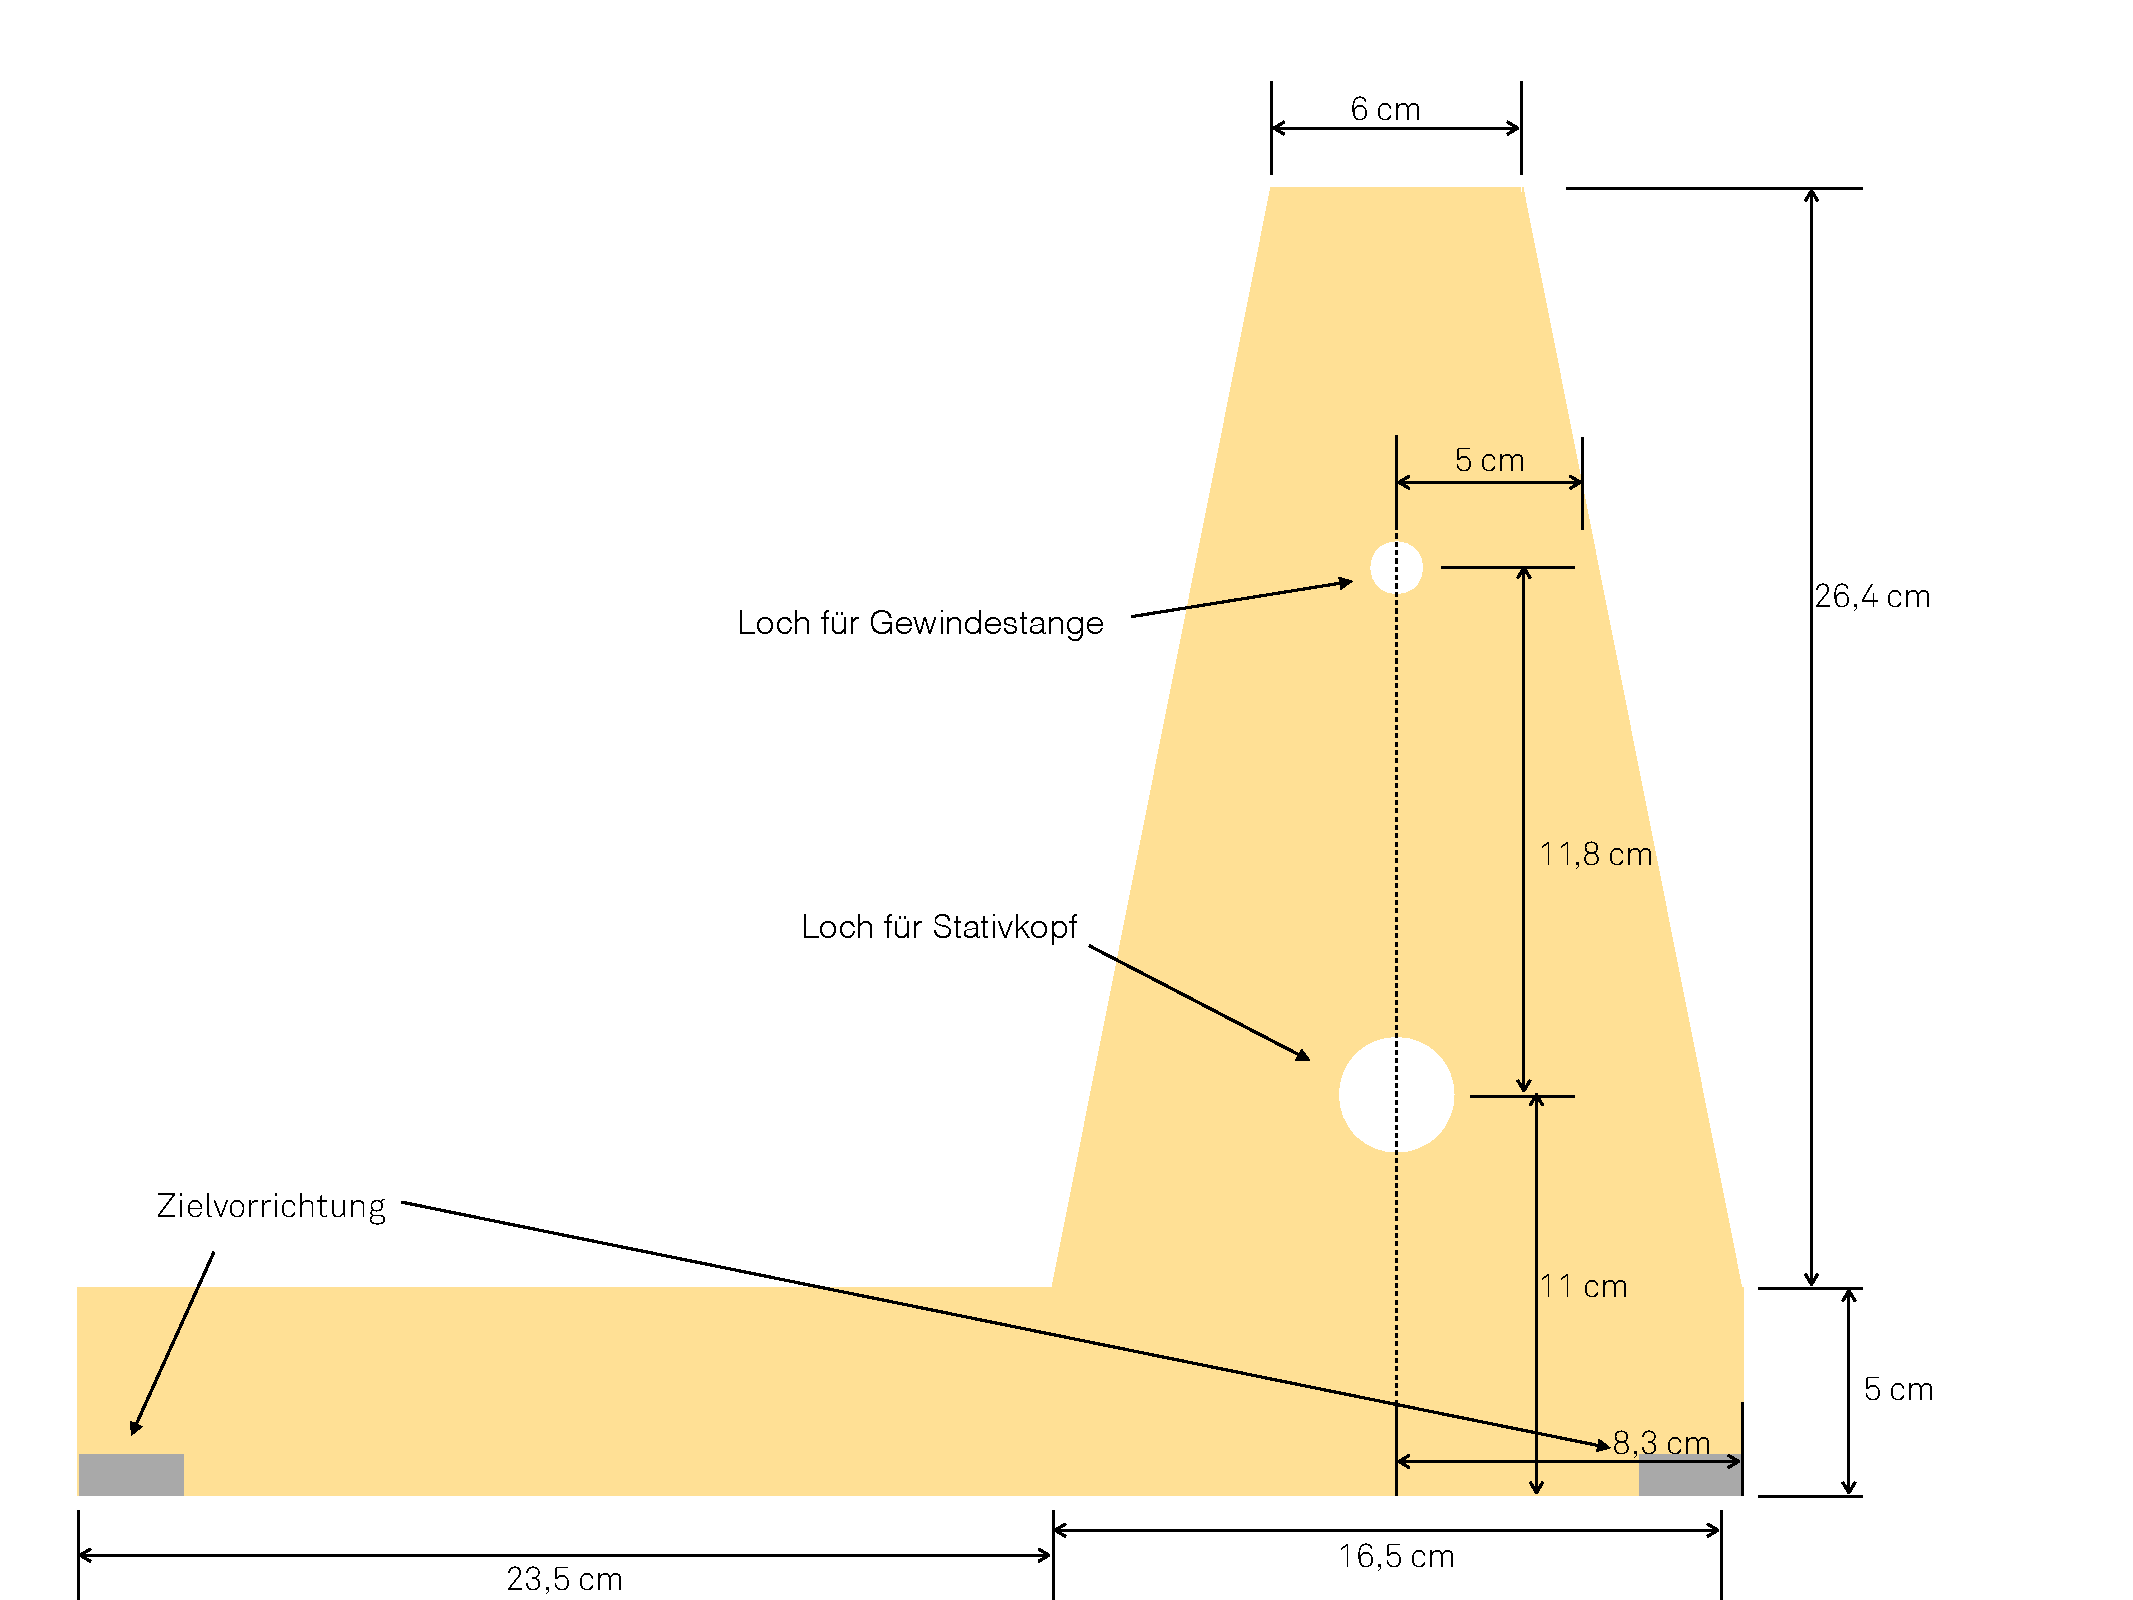
\includegraphics[width=\linewidth]{images/NachfuehrungSchemaOben.pdf}%
    \caption{Obere Sperrholzplatte.}
  \end{subfigure}
  \begin{subfigure}{0.75\columnwidth}
    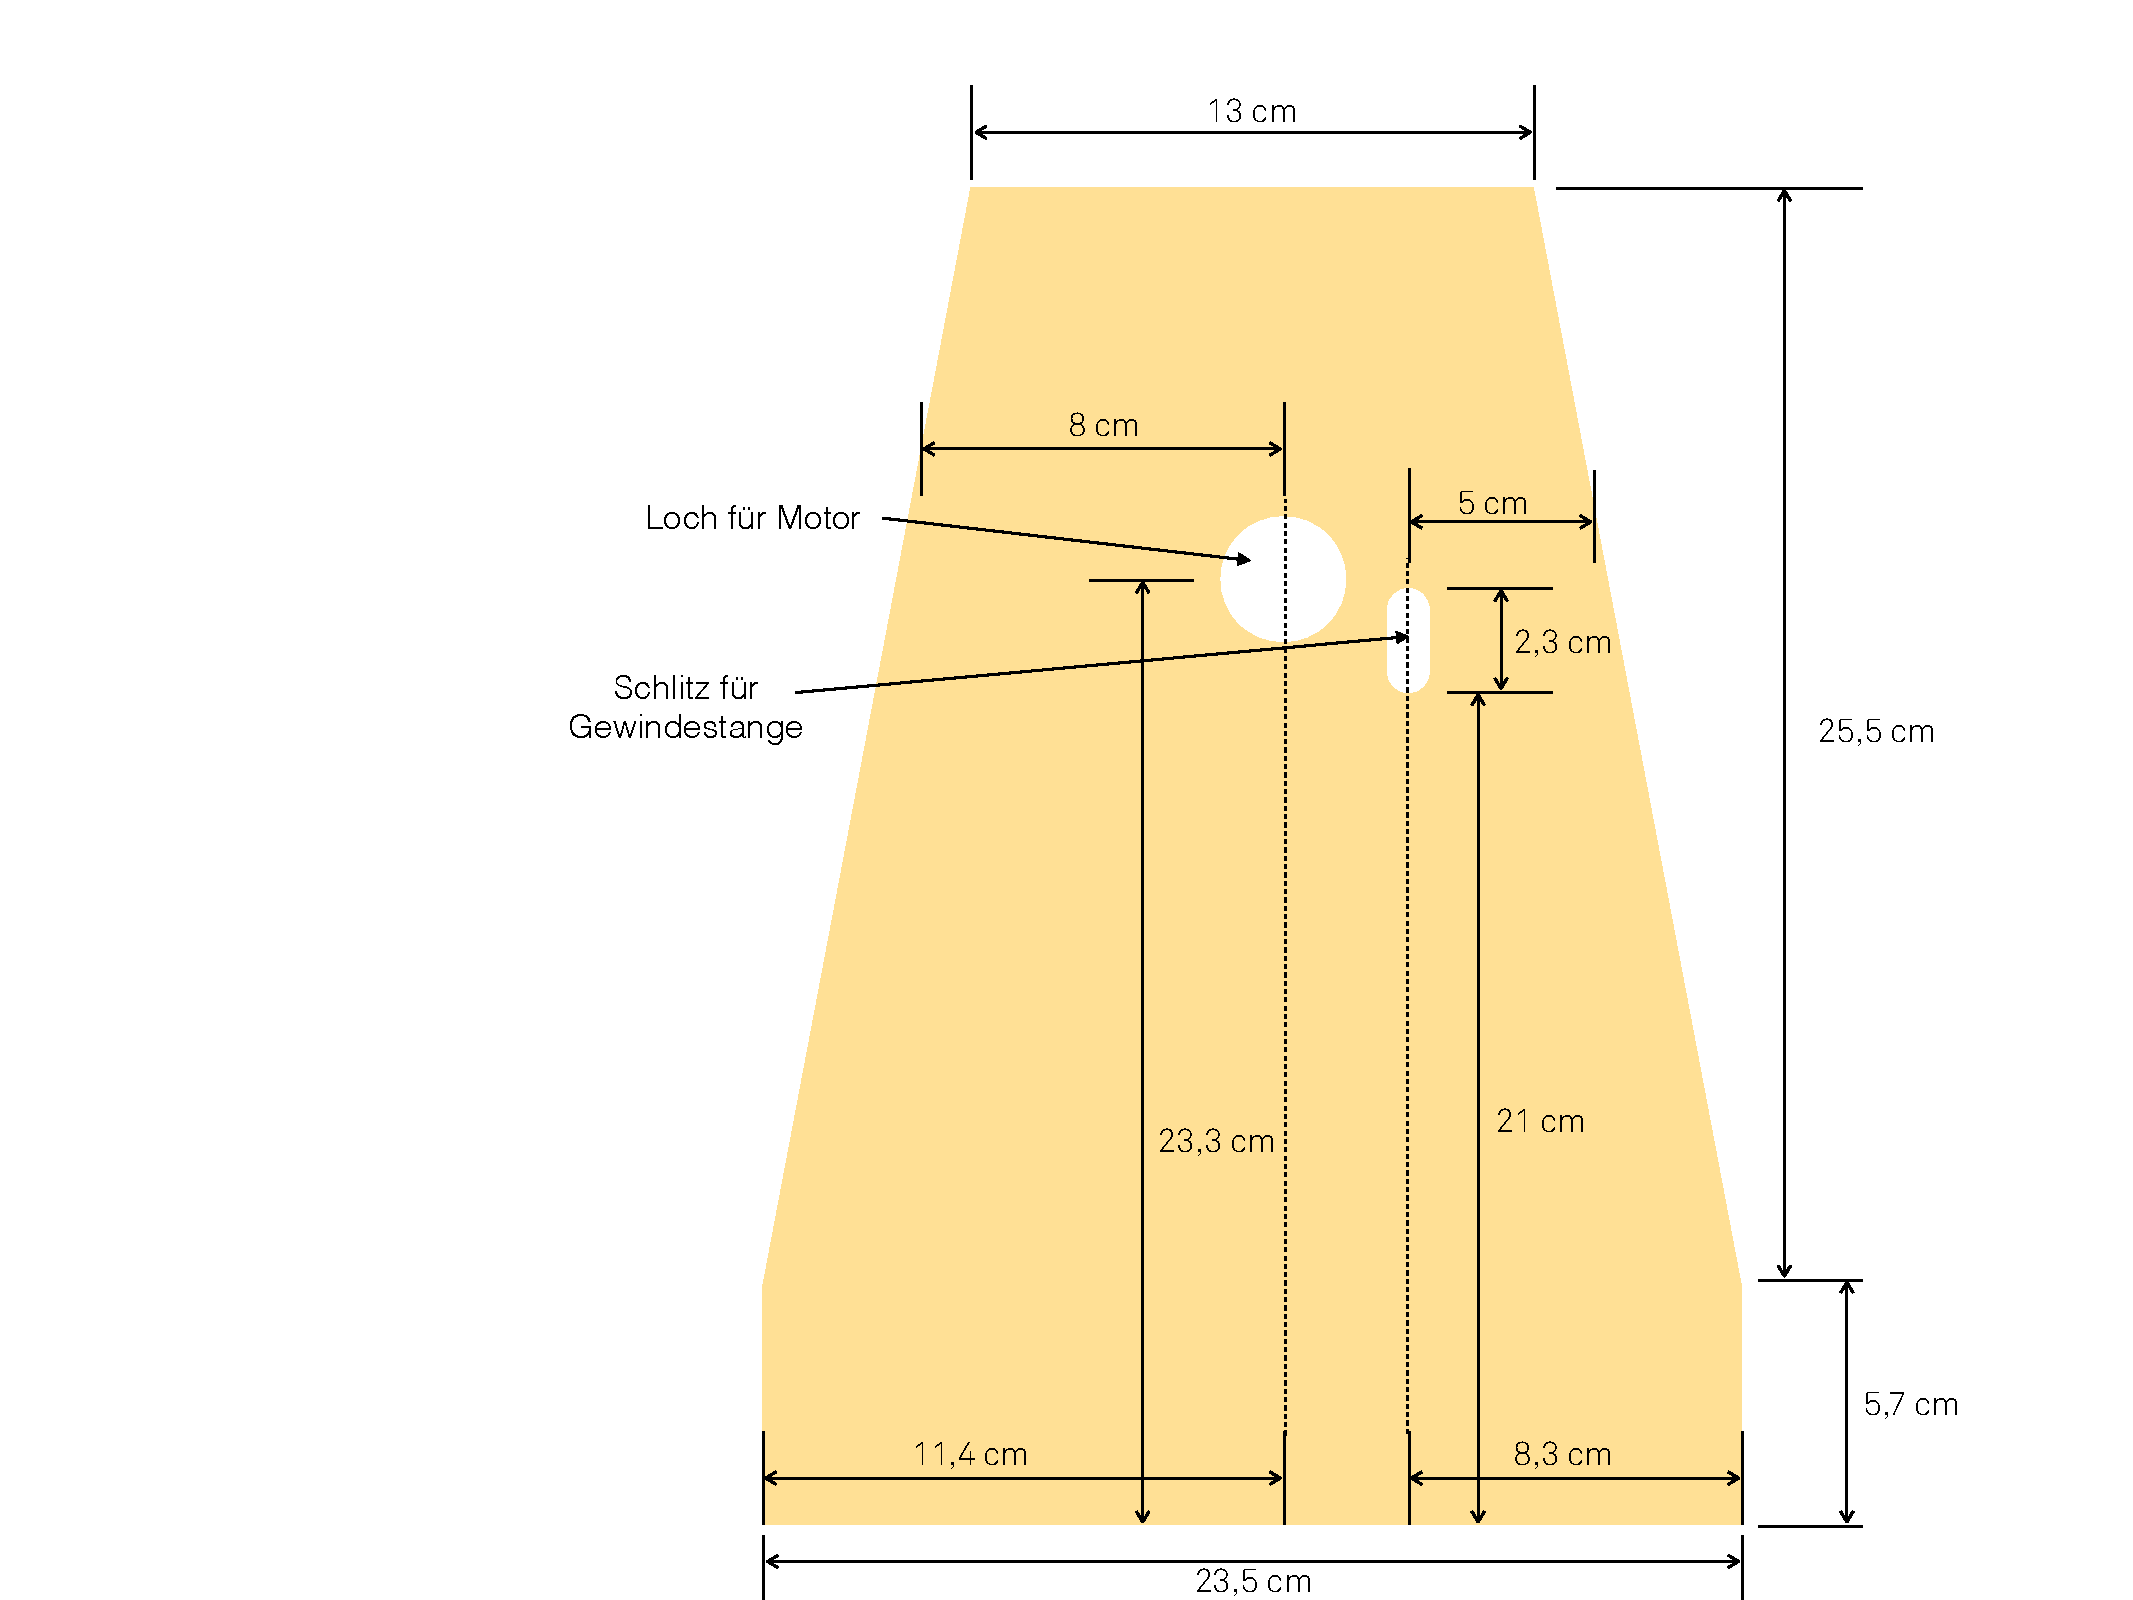
\includegraphics[width=\linewidth]{images/NachfuehrungSchemaUnten.pdf}%
    \caption{Untere Sperrholzplatte.}
  \end{subfigure}
  \caption{Zeichnung der beiden Sperrholzplatten.}%
  \label{fig:schema}
\end{figure}

Zur Veranschaulichung sind in Abbildung~\ref{fig:schema} die beiden Sperrholzplatten maßstrabsgetreu dargestellt.
Ein Foto der fertigen Nachführung ist in Abbildung~\ref{fig:barndoor} zu sehen.


\subsection{Durchführung}
Die Rotationsachse verläuft entlang der Scharniere und muss vor den Aufnahmen auf den Himmelsnordpol in der Nähe des Polarsterns ausgerichtet werden, um die Rotation bezüglich des Sternenhimmels auszugleichen.
Zudem muss die Motorgeschwindigkeit angepasst werden.
Bei korrekter Einstellung dreht sich das große Zahnrad mit einer Umdrehung pro Minute.

\subsection{Ergebnisse}
Aufgrund des bewölkten Himmels konnten leider nur wenige Aufnahmen gemacht werden, Abbildung~\ref{fig:milkyway} zeigt eine Weitwinkelaufnahme des Sternenhimmels. 
Die Ausläufer der Milchstraße sind deutlich zu erkennen und die Belichtungszeit von acht Minuten hätte ohne die Nachführung zu deutlichen Strichspuren bei den Sternen geführt.
\begin{figure}
  \centering
  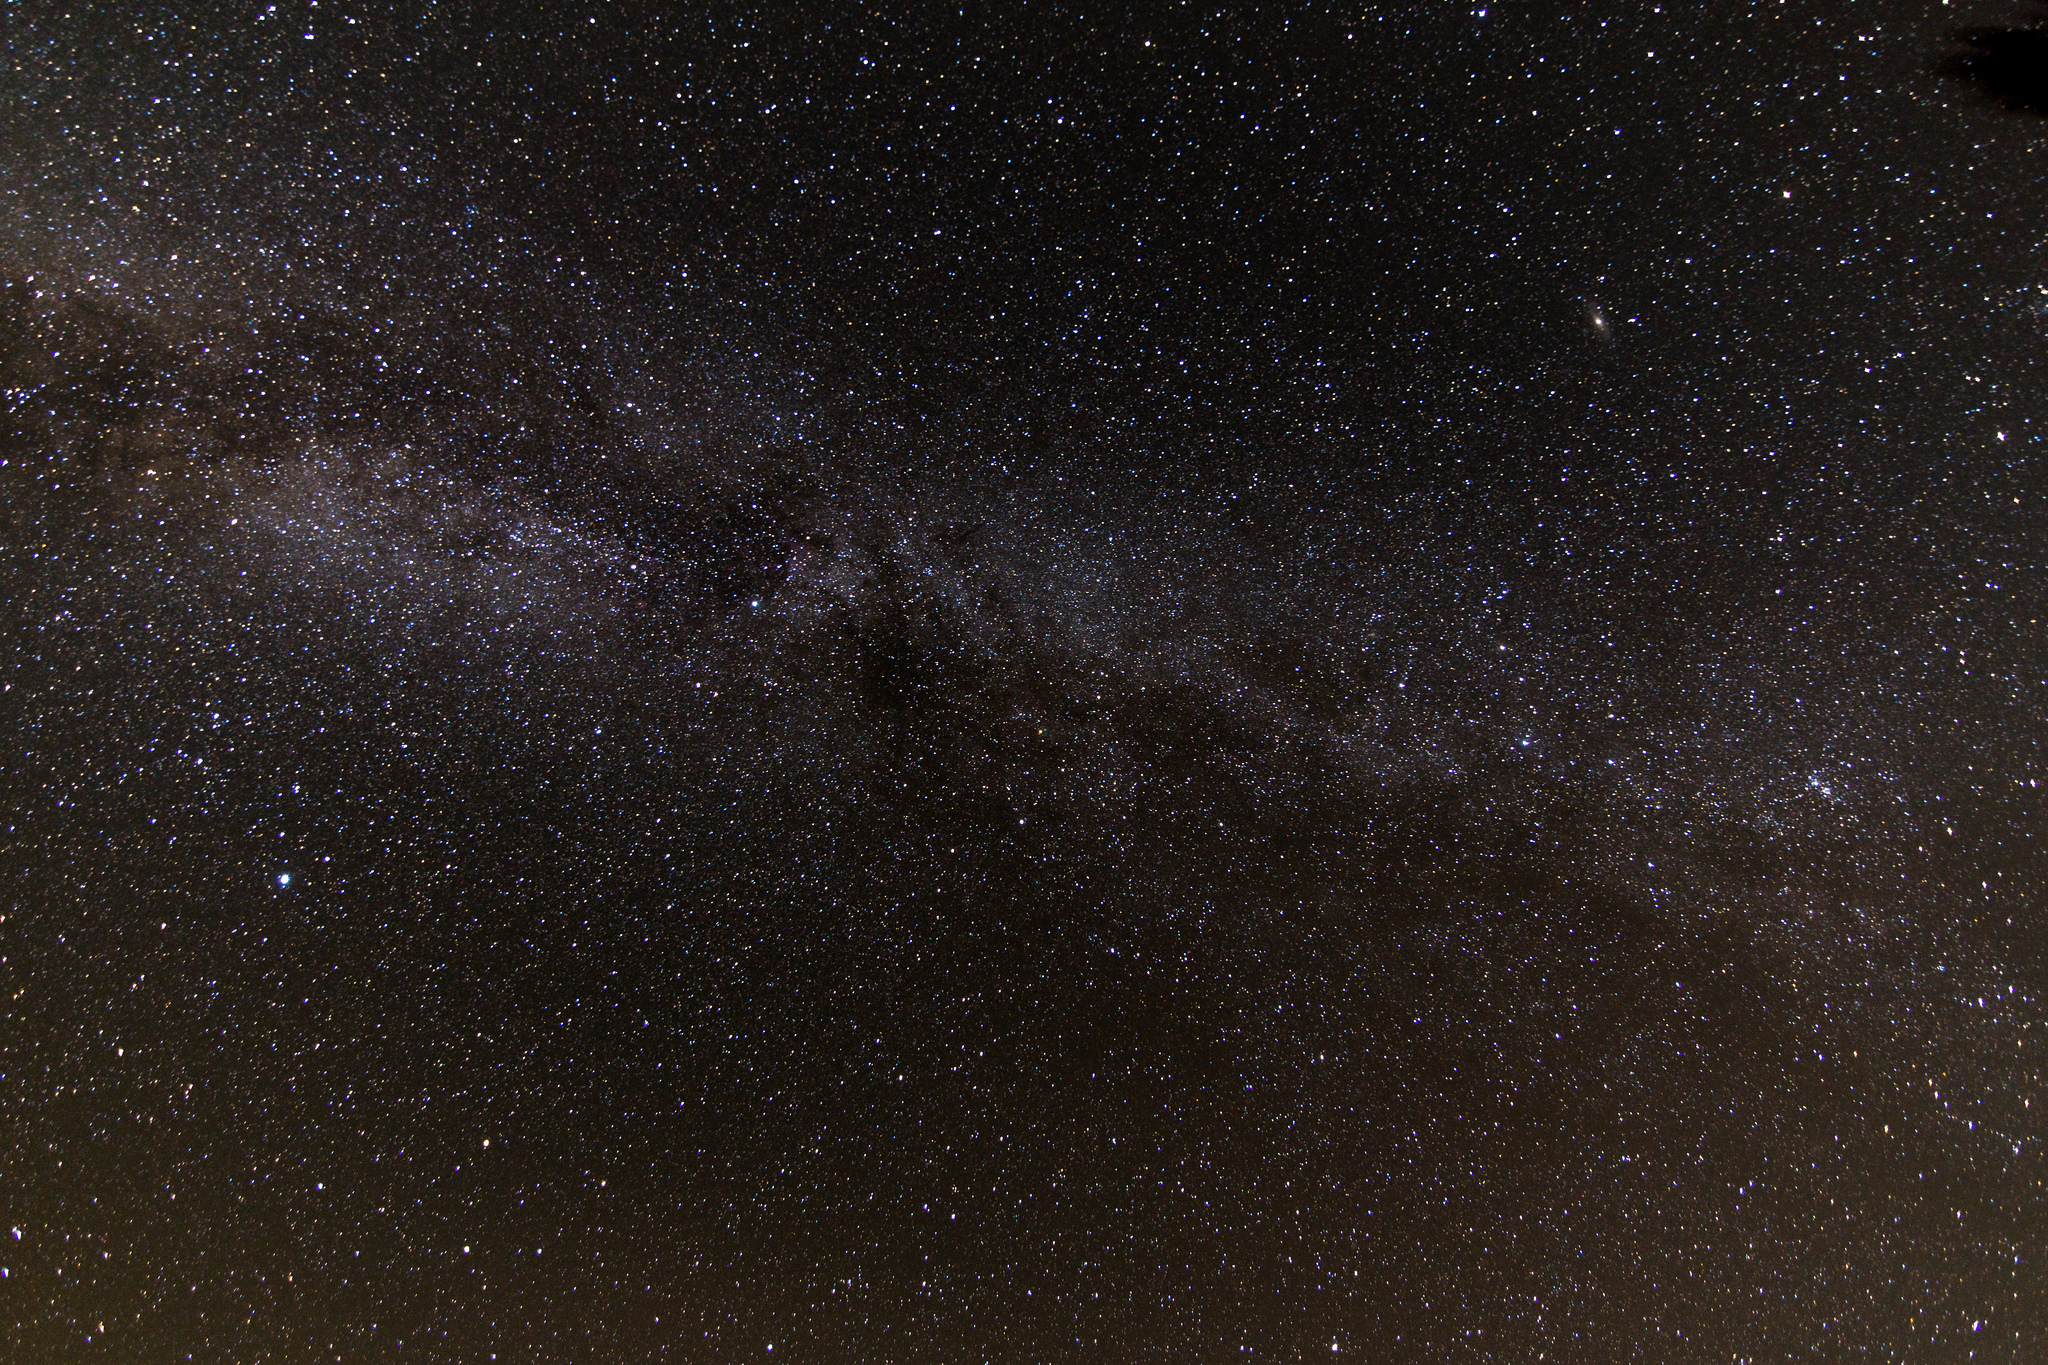
\includegraphics[width=\linewidth]{images/milkyway.jpg}
  \caption{Weitwinkelaufnahme des Himmels über Tschagguns, Belichtungszeit: \SI{8}{\minute}, Blende \num{2.8}, Brennweite \SI{11}{\milli\metre}, Kamera: \textsc{Sony Alpha 77}.}
  \label{fig:milkyway}
\end{figure}

\subsection{Probleme und Verbesserungsmöglichkeiten}

Die Gewindestange hat keine ideale Krümmung und ist an manchen Stellen stärker
gekrümmt als an anderen. Dies führt dazu, dass sich die Sterne auf den Bildern
in nicht-zyklischen Figuren bewegen. 

Weiterhin ließe sich die Zielvorrichtung verbessern: mit der hier verwendeten Konstruktion ist das Anvisieren des Himmelnordpols bei Dunkelheit schwierig, da man die Umrisse des hinteren Ziellochs nicht erkennen kann.

\section{Nebelkammer}

\subsection{Material}
Hat Vukan


\subsection{Aufbau}
Zu Beginn wurde aus den Glasplatten mithilfe von Silikon ein Aquarium gebaut.
Danach wurde der Styroporblock halbiert und übereinander befestigt. In den
oberen Block wurde eine Öffnung in der Größe der Metallplatte hereingeschnitten.
Die Metallplatte wurde mit schwarzem Klebenband beklebt, um einen möglichst
großen Kontrast zu ermöglichen. Als letzer Schritt des Aufbaus wurde das Filz
passend zugeschnitten und mithilfe von Magneten an der Unterseite des Aquariums
befestigt.

\subsection{Durchführung}
Um unsere Nebelkammer funktionsbereit zu machen, wurde der Filz in Isopropanol
getränkt. Des Weiteren wurde der Hohlraum im Styroporblock mit Trockeneis
gefüllt und die Metallplatte eingesetzt. Auf die Platte wurde das Aquarium
mithilfe von Knete luftdicht angebracht. Durch das Isopropanol an der Oberseite
entstand ein feiner Nebel, in dem Spuren von Teilchen beobachtet werden können.
Um die Nebelerzeugungsprozeß zu beschleunigen, kann die Oberseite mithilfe eines
Föhns erwärmt werden.

\subsection{Ergebnisse}
Es konnten zahlreiche Teilchenspuren beobachtet werden. (Video)

\subsection{Probleme und Verbesserungen}
Probleme, welche die Funktion der Nebelkammer stark unterbinden, traten nicht
auf. Jedoch gibt es zahlreiche Verbesserungsmöglichkeiten. Das Schneiden von
Styropor mithilfe von Cuttermessern und Sägen ist nicht optimal. Besser und
vorallen sauberer kann Styropor mit einem heißem Draht geschnitten werden. Das
Verkleben der Glaspaltten mit Silikon ist eine große Sauerei und kann durch den
Kauf eines bereits fertigen Aquariums umgangen werden. Für einen optimalen
Kontrast könnte die Metallplatte schwarz lackiert oder direkt eine schwarze
Platte verwendet werden. Das schwarze Klebeband erfüllt diesen Zweck nur
befriedigend. Verbesserungen können ebenfalls bei der Abdichtung zwischen der
Metallplatte und dem Aquarium erfolgen. Die verwendete Knete erfüllt diesen Job
nicht zufrieden stellend. Es kam durch diese Undichtigkeiten zu einem Luftzug
innerhalb der Nebelkammer, wodurch die Teilchen-Spuren nicht optimal detektiert
werden konnten. Als Alternative zur Knete könnten passende Gummidichtungen
verwendet werden. Des Weiteren könnte die Verbindung auch mit Silikon erfolgen.
Nachteil wäre dann, dass das Aquarium dauerhaft verbunden wäre. Zur Verbesserung
könnte das Aquarium auch mit einem dicht schließenem Deckel ausgestattet werden.
Als Trockeneis-Alternative könnte ein Peltier-Element benutzt werden.

\section{Solarkocher}
\section{Solarofen}
\section{Wasserrakete}
\end{document}

